% 手工维护（不由 tools/convert.sh 生成）：来源 doc/readme/tiny210/memory-layout.md
\chapter[内存布局与 \texttt{/proc} 内存信息]{内存布局与 /proc/meminfo、/proc/iomem}\label{ch:memory-layout}

本章说明 \texttt{tiny210} 分支 ARM32 内核的内存布局：物理 RAM、内核镜像、页分配器、
MMIO 外设区、用户与内核虚拟地址空间，以及 Linux 风格的 \texttt{/proc/meminfo}、
\texttt{/proc/iomem} 如何把它们显示出来。数值按\textbf{实板}（DRAM 起始 0x20000000）给出；
QEMU 替身（cubieboard，DRAM 起始 0x40000000）结构相同，只是基址不同。
图~\ref{fig:memory-layout} 把四者画在同一张图上。

\begin{figure}[p]
\centering
\rotatebox{90}{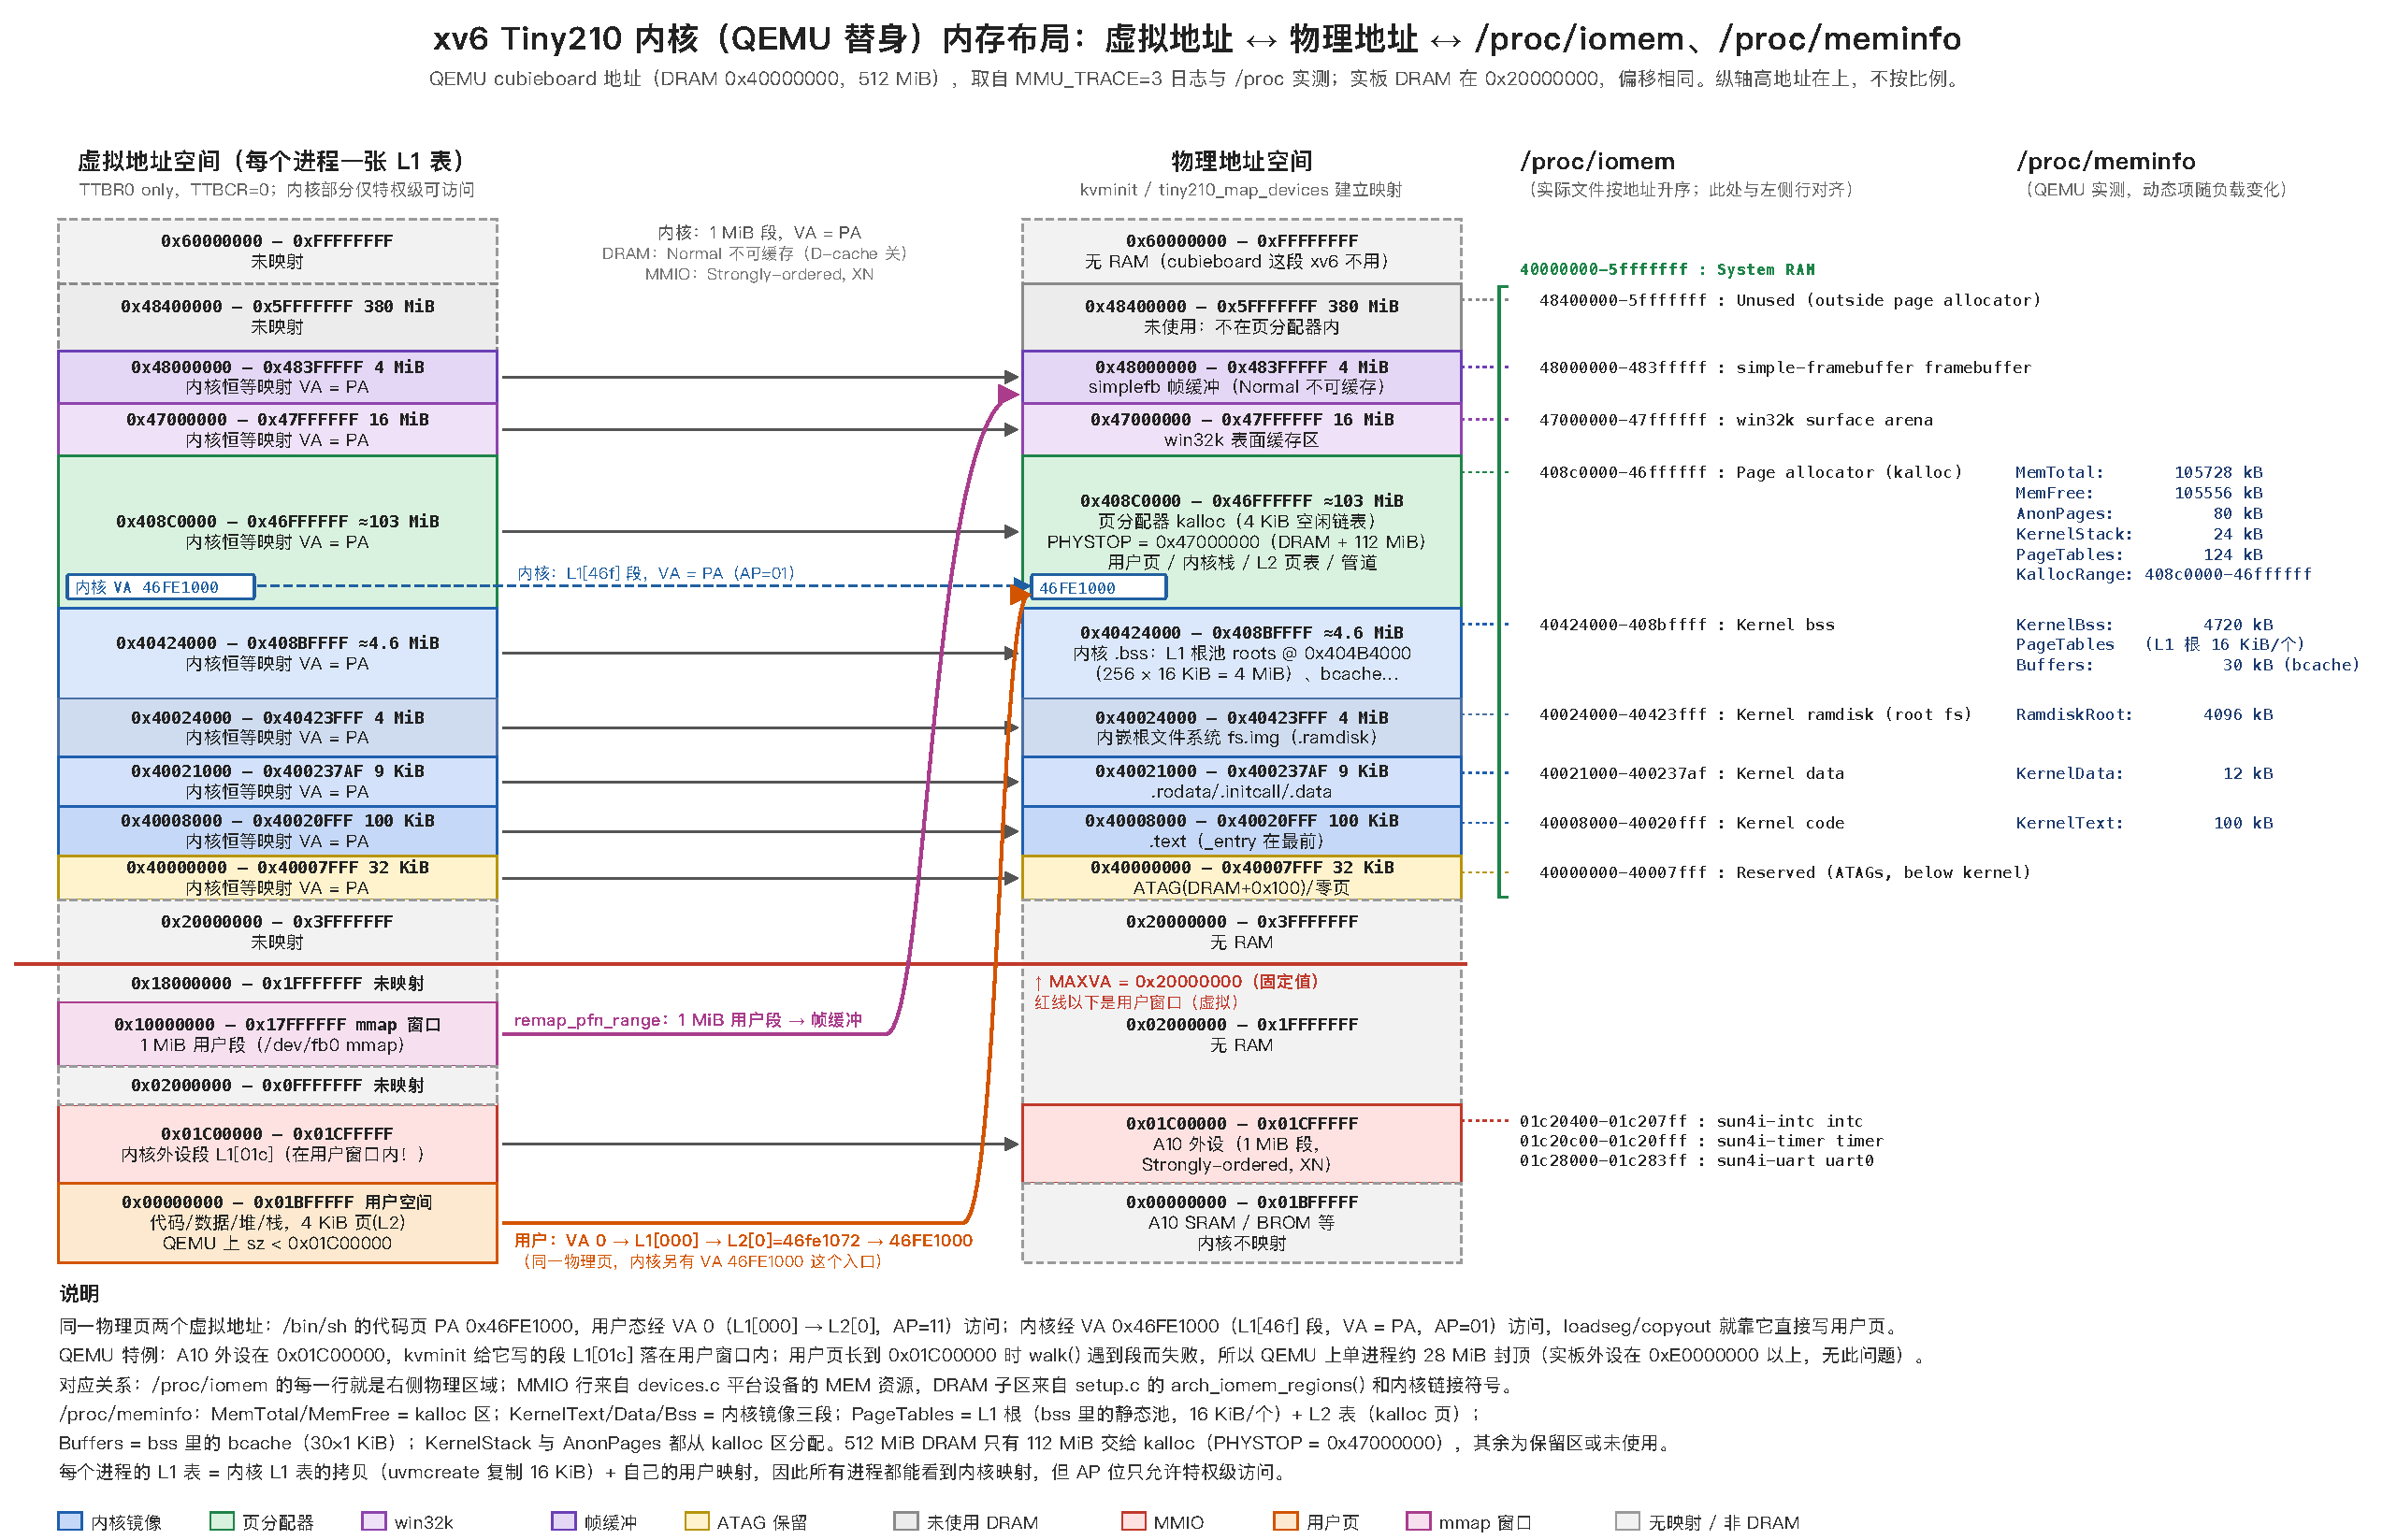
\includegraphics[width=0.92\textheight,height=\textwidth,keepaspectratio]{figures/memory-layout.pdf}}
\caption{虚拟地址 $\leftrightarrow$ 物理地址 $\leftrightarrow$ \texttt{/proc/iomem}、\texttt{/proc/meminfo}
（QEMU 地址：DRAM 从 0x40000000 开始，数值取自 MMU\_TRACE 日志与 /proc 实测；实板偏移相同、基址为 0x20000000。高地址在上，不按比例；由 \texttt{tools/memory\_layout\_svg.py} 生成）}\label{fig:memory-layout}
\end{figure}

\section{物理内存}

\begin{longtable}{@{}>{\raggedright\arraybackslash}p{0.2\textwidth}>{\raggedright\arraybackslash}p{0.37\textwidth}>{\raggedright\arraybackslash}p{0.37\textwidth}@{}}
\toprule
区域 & 实板地址 & 来源 \\
\midrule
\endhead
DRAM bank 0 & 0x20000000--0x3fffffff（512 MiB） & ATAG\_MEM（BL1 或 QEMU 传入），\texttt{board.h} 的 \texttt{BOARD\_DRAM\_SIZE} 兜底 \\
ATAG / 零页 & DRAM+0x0 -- DRAM+0x7fff & BL1 把 ATAG 放在 DRAM+0x100，内核不回收 \\
内核镜像 & 0x20008000 起 & Linux \texttt{TEXT\_OFFSET} 约定，\texttt{kernel.ld} 的 \texttt{KERNEL\_LOAD} \\
页分配器 & \texttt{end} -- DRAM+112 MiB & \texttt{setup.c}：\texttt{USE\_DRAM = S5PV210\_USE\_DRAM} \\
win32k 表面缓存区 & DRAM+112 MiB -- +128 MiB & \texttt{memlayout.h} 的 \texttt{S5PV210\_GUI\_*}，不交给 kalloc \\
LCD 帧缓冲 & DRAM+128 MiB -- +132 MiB & \texttt{devices.c} 中 s3c-fb 的 framebuffer 资源 \\
未使用 & DRAM+132 MiB -- DRAM 顶 & 约 380 MiB 闲置 \\
\bottomrule
\end{longtable}

\begin{itemize}
\item \textbf{512 MiB 中只有 112 MiB 用作通用内存。} D-cache 关闭时 \texttt{kinit} 逐页初始化很慢，
      所以 \texttt{PHYSTOP = DRAM\_BASE + 112 MiB}，ATAG 报告的其余内存不进分配器。
\item \texttt{PHYSTOP} 实际是变量 \texttt{tiny210\_phystop}：ATAG 报告的 bank 更小时会下调；
      内核本身超过它时会上调到 \texttt{end + 16 MiB}。
\end{itemize}

\section{内核镜像}

下表是实板构建的链接符号（\texttt{arm-none-eabi-nm kernel.elf}）：

\begin{longtable}{@{}>{\raggedright\arraybackslash}p{0.27\textwidth}>{\raggedright\arraybackslash}p{0.3\textwidth}>{\raggedright\arraybackslash}p{0.1\textwidth}>{\raggedright\arraybackslash}p{0.27\textwidth}@{}}
\toprule
段 & 地址 & 大小 & 内容 \\
\midrule
\endhead
Kernel code（.text） & 0x20008000--0x2002efff & 156 KiB & \texttt{\_entry} 在最前（\texttt{.text.entry}） \\
Kernel data（.rodata/.initcall/.data） & 0x2002f000--0x2003ffff & 68 KiB & 含 MT7601U 固件 45 KiB \\
Kernel bss & 0x20040000--0x20539fff & 约 5 MiB & 见下 \\
\bottomrule
\end{longtable}

bss 的大头：
\begin{itemize}
\item \texttt{roots}：\textbf{4 MiB}，256 个 16 KiB 对齐的 ARMv7 L1 页表根的静态池（\texttt{vm.c}），
      这也是地址空间个数（进程数）的上限；
\item \texttt{fw\_buf} 256 KiB、\texttt{diskmap} 256 KiB（FAT32 簇表）、\texttt{tcp\_connections} 220 KiB、
      \texttt{mt\_rx\_buf} 64 KiB；
\item \texttt{bcache}：30 个 1 KiB 块缓存（\texttt{NBUF = MAXOPBLOCKS*3}）。
\end{itemize}
QEMU 构建额外把根文件系统 \texttt{fs.img} 链接进 \texttt{.ramdisk} 段（4 MiB），位于 data 与 bss 之间。

\section{页分配器}

\texttt{kernel/kalloc.c} 是一条 4 KiB 页的单链表 freelist，一把自旋锁，没有 buddy，也没有 slab。
管理范围是 \texttt{[PGROUNDUP(end), PHYSTOP)}，实板约 0x2053a000--0x26ffffff，即
\textbf{106.8 MiB}（109336 kB）；QEMU 实测 0x408c0000--0x46ffffff = 105728 kB。

从 kalloc 取页的有：内核栈（每进程 1 页）、用户页、L2 页表、管道缓冲、\texttt{/proc} 读缓冲。
每个 L2 页表占一整页，但 ARMv7 的 L2 表只有 1 KiB，所以每张浪费 3 KiB。L1 根不来自 kalloc，
来自上面的静态池。kalloc 维护 \texttt{nfree}、\texttt{managed} 计数和 \texttt{[lo, hi)} 范围，
供 \texttt{kmemstat()} 读取，\texttt{kfreepages()} 不再遍历整条链表。

\section{MMIO 外设区}

所有 MMIO 都按 \texttt{devices.c} 平台设备表中的 MEM 资源映射为 1 MiB 段
（\texttt{tiny210\_map\_devices()}），属性是 Strongly-ordered、XN、仅特权级可访问：

\begin{longtable}{@{}>{\raggedright\arraybackslash}p{0.2\textwidth}>{\raggedright\arraybackslash}p{0.3\textwidth}>{\raggedright\arraybackslash}p{0.44\textwidth}@{}}
\toprule
设备 & 物理地址 & 说明 \\
\midrule
\endhead
s5pv210-clock & 0xE0100000（64 KiB） & 同一段里还有 SWRESET 0xE0102000、PS\_HOLD 0xE010E81C、USB\_PHY\_CONTROL \\
s5pv210-gpio / keys & 0xE0200000（4 KiB） & GPIO、EINT16--31 按键 \\
s5pv210-pwm & 0xE2500000 & 时钟源 timer3，tick 用 timer4（IRQ 25） \\
s3c2410-wdt & 0xE2700000 & 看门狗 \\
s5pv210-uart & 0xE2900000 & UART0 控制台 \\
s3c-sdhci & 0xEB000000 + 1 MiB$\times$通道 & 启动 SD 通道（由 iROM 变量 0xD0037488 决定） \\
s3c-hsotg（可选） & 0xEC000000 & \texttt{S5PV210\_USB\_OTG=1} 时启用 \\
USB PHY & 0xEC100000 & EHCI 与 OTG 共用 \\
s5p-ehci & 0xEC200000（IRQ 55） & USB-A 主机口 \\
s5pv210-vic & 0xF2000000（4 MiB） & VIC0--3 \\
s3c-fb（FIMD） & 0xF8000000 & LCD 控制器 \\
\bottomrule
\end{longtable}

BL1 运行的 iRAM（0xD0020000）只在 MMU 打开前访问，不做映射。QEMU 版换成 Allwinner A10 的外设：
intc 0x01C20400、timer 0x01C20C00、uart0 0x01C28000。

\section{虚拟地址空间}

使用 ARMv7 短描述符页表，\textbf{只用 TTBR0}（TTBCR=0）。内核与用户共用一张 L1 表，
\textbf{内核恒等映射}（\texttt{V2P(a)=a}，\texttt{KERNBASE=0}）：

\begin{lstlisting}
0x00000000 +--------------------------+
           | user text/data/heap/stack|  4 KiB pages (L2), sz < 32 MiB (uvmalloc limit)
0x02000000 +--------------------------+
           | (unmapped)               |
0x10000000 +--------------------------+
           | mmap window              |  user 1 MiB sections (/dev/fb0), shared by fork
0x18000000 +--------------------------+
           | (unmapped)               |
0x20000000 +==========================+  MAXVA = DRAM_BASE: end of the user window
           | DRAM identity (0-112 MiB)|  1 MiB sections, privileged, Normal non-cacheable
           | win32k arena, framebuffer|  1 MiB sections
0xE0000000 +--------------------------+
           | peripheral MMIO sections |  Strongly-ordered, XN, privileged
0xFFFFFFFF +--------------------------+
\end{lstlisting}

\begin{itemize}
\item \texttt{uvmcreate()} 把内核 L1 表整张（16 KiB）复制进每个进程的根，
      所以每个进程都有内核映射，靠 AP 位挡住用户态访问。
\item \texttt{\_Static\_assert(DRAM\_BASE >= MAXVA)} 保证用户窗口不会与内核恒等映射重叠；
      这也是为什么 QEMU 的 DRAM 在 0x40000000，用户窗口却仍只到 0x20000000。
\item 缓存：I-cache 和分支预测开启，\textbf{D-cache 关闭}。DRAM 段的属性是 TEX=001、C=0、B=0（Normal、不可缓存）。
      \texttt{devices.c} 里 \texttt{SECTION\_RAM} 的注释写着 ``cached Normal memory''，
      但它的位编码与 DRAM 段相同，实际同样不可缓存。
\end{itemize}

\subsection{kvminit() 图解：两级页表}

Cortex-A8 没有 LPAE，短描述符最多两级。图~\ref{fig:mmu-page-tables} 仿照 minios 的
\texttt{\_\_create\_page\_tables} 图解画出 Tiny210 的情况：左上是代码 ①--⑧，右上是两种描述符
（L1 段、L1 表描述符 + L2 小页），中间按 VA $\rightarrow$ L1 $\rightarrow$ L2 $\rightarrow$ PA 画出结果，
下面是 \texttt{install()} 的寄存器写入和注意事项。内核只用 L1 段（共 145 个：DRAM 112、win32k 16、
帧缓冲 4、MMIO 13）；用户窗口的 L1 项是 01 型表描述符，指向 \texttt{walk()} 从 kalloc 取的 L2 表，
L2 项 \texttt{PA|0x72} 映射 4 KiB 小页。

\begin{figure}[p]
\centering
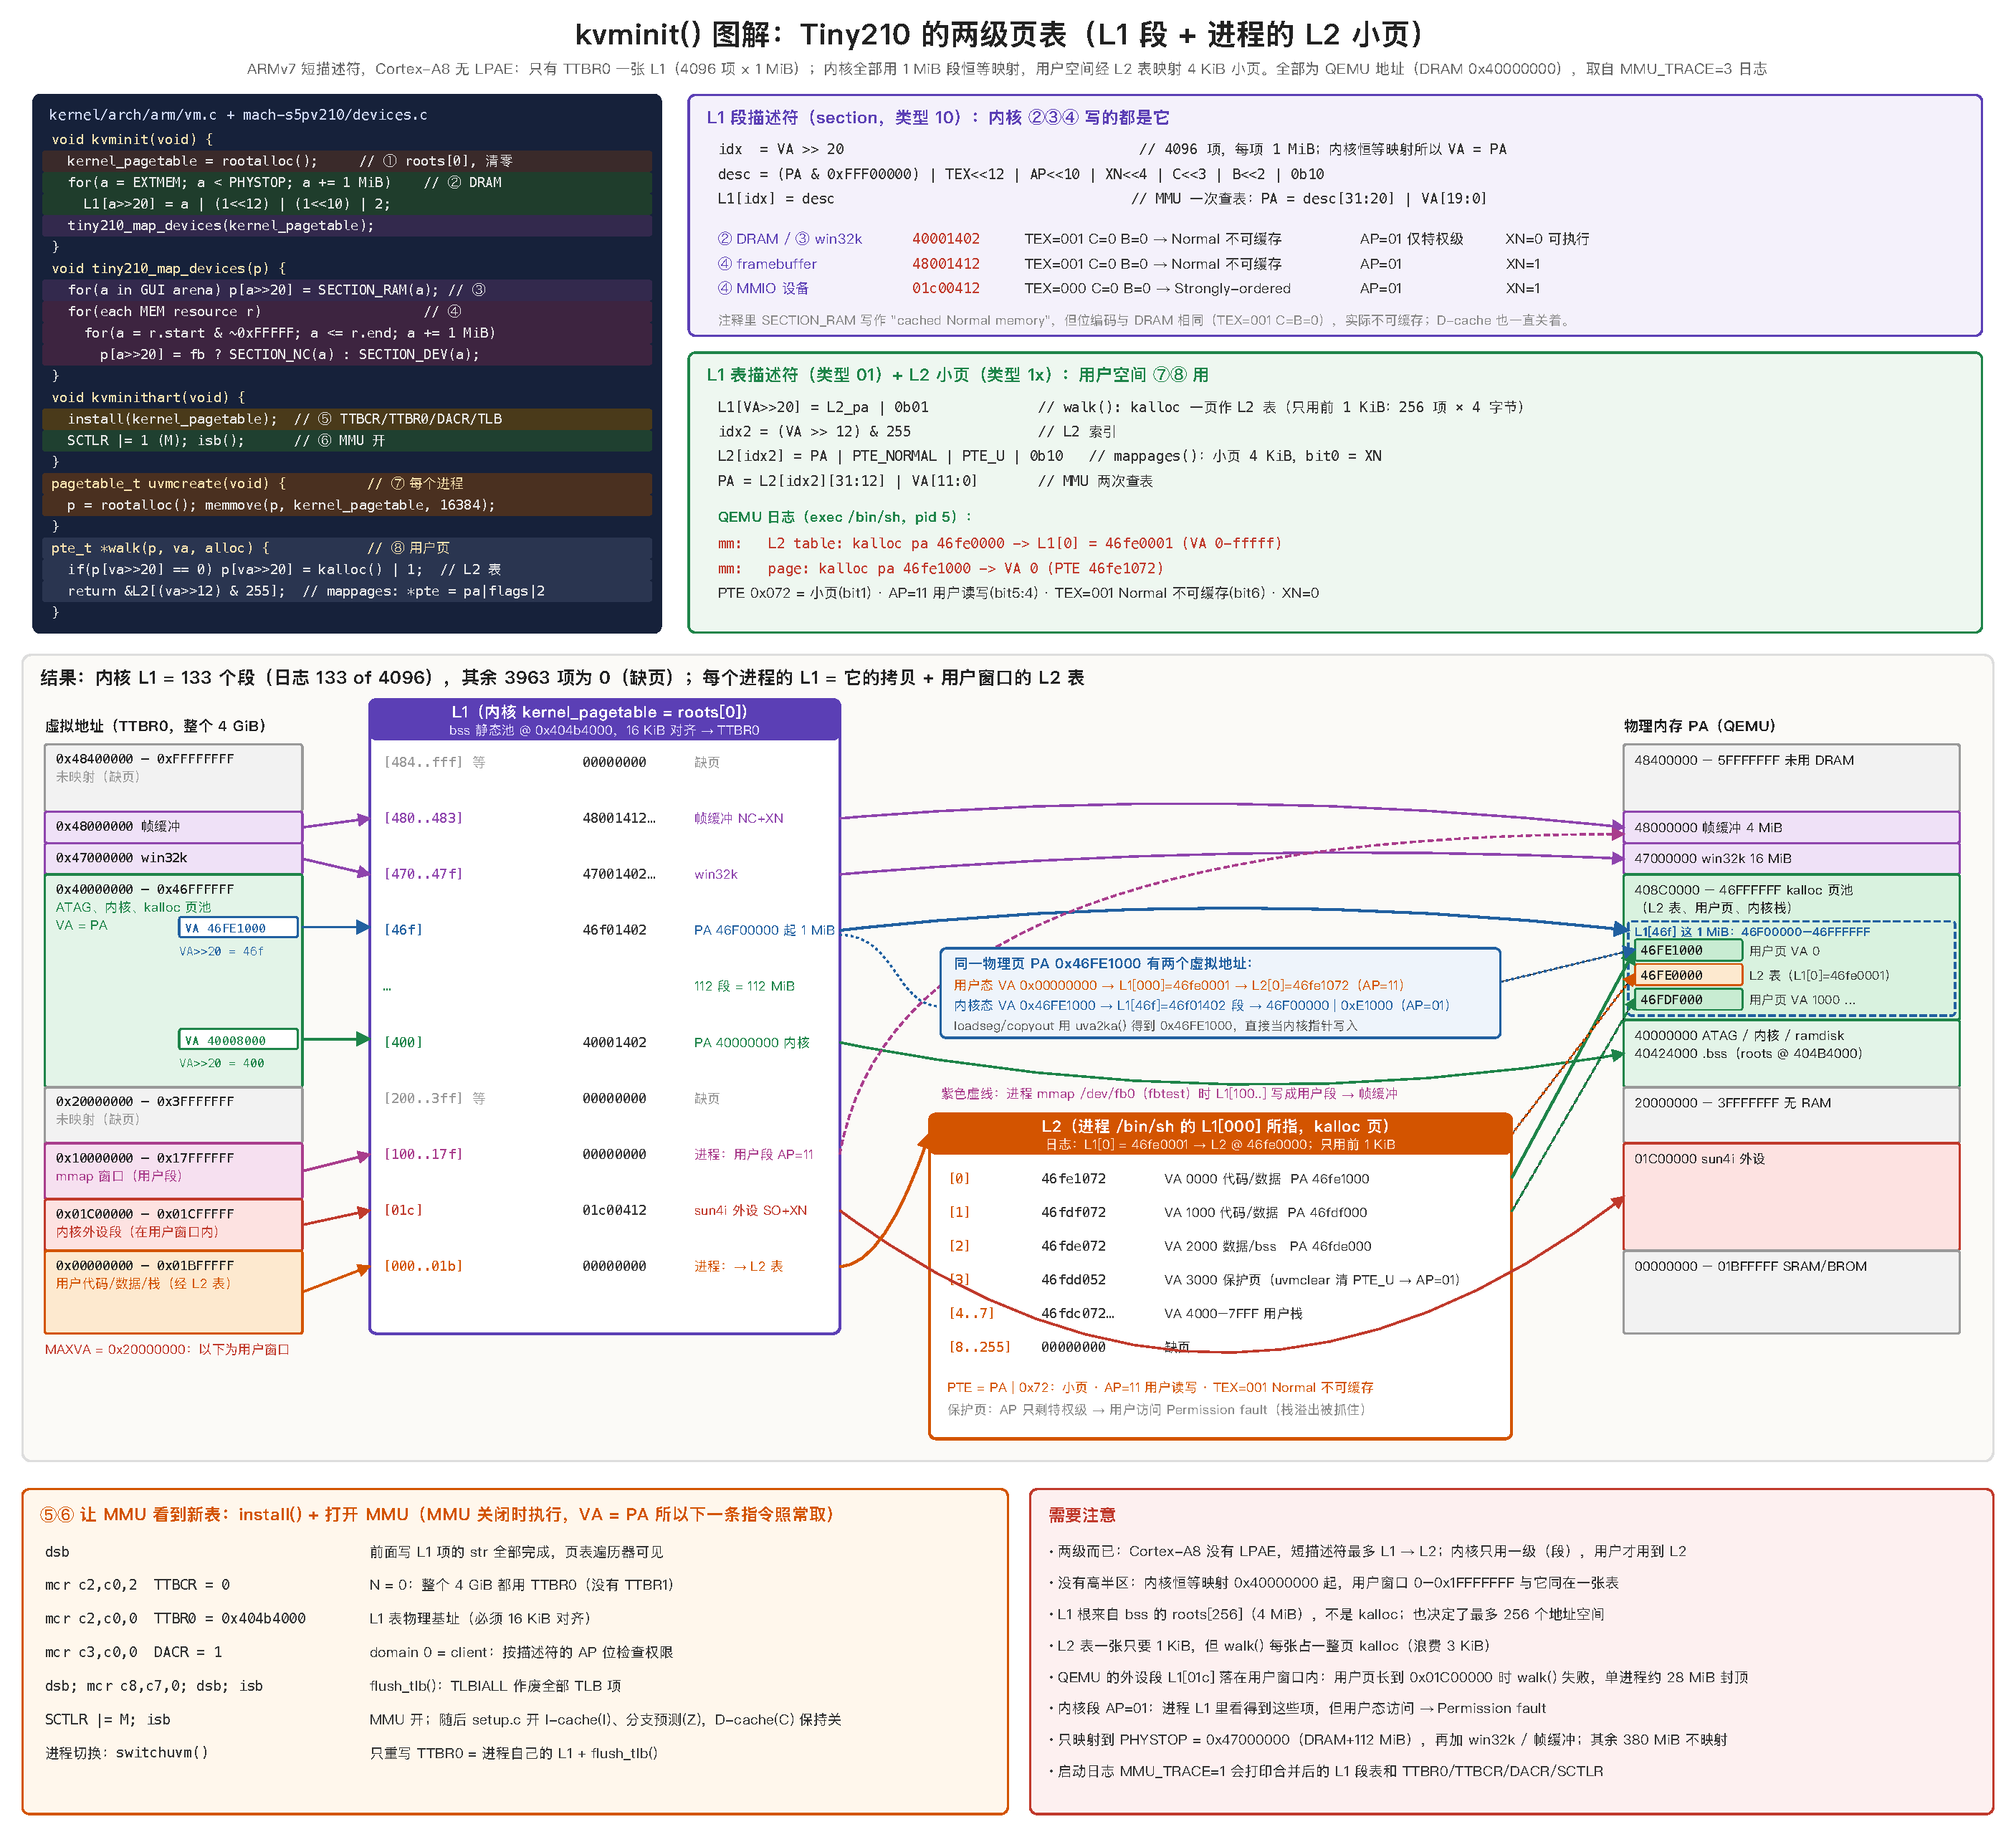
\includegraphics[width=\textwidth,height=0.92\textheight,keepaspectratio]{figures/mmu-page-tables.pdf}
\caption{kvminit() 图解：内核 L1 段与进程的 L2 小页（QEMU 地址；\texttt{tools/mmu\_page\_tables\_svg.py} 生成）}\label{fig:mmu-page-tables}
\end{figure}

\subsection{页表本身放在物理内存哪里}

\begin{itemize}
\item \textbf{内核 L1} 就是 \texttt{roots[0]}。\texttt{roots[256][4096]} 是 \texttt{vm.c} 的静态数组，位于内核
      \textbf{.bss}，不来自 kalloc：实板 roots 池在 0x200D4000--0x204D3FFF，开机 TTBR0 = 0x200D4000
      （QEMU 为 0x404B4000）。
\item \textbf{进程 L1}：\texttt{uvmcreate()} 调 \texttt{rootalloc()} 在\textbf{同一个 roots 池}里取空槽 roots[k]，
      再 \texttt{memmove} 整张 16 KiB；地址 = roots 基址 + k$\times$0x4000（QEMU 日志：/bin/sh 用 roots[6] = 0x404CC000）。
      \texttt{uvmfree} 只把 \texttt{used[k]} 清 0，不经过 kalloc。
\item \textbf{L2 表}：\texttt{walk()} 发现 L1 项为 0 时 \texttt{kalloc()} 一页，位于 \textbf{kalloc 页池}
      （实板 0x2053A000--0x26FFFFFF）。freelist 后进先出，kinit 按地址升序 kfree，表头是最高地址的页，
      所以最早分配的 L2 表和用户页紧贴 PHYSTOP 下方（QEMU：L2 在 0x46FE0000，用户页 0x46FE1000 起）。
\end{itemize}

\section{/proc/meminfo 与 /proc/iomem}

实现在 \texttt{kernel/memstat.c}，由 \texttt{kernel/vfs.c} 的 procfs 调用：
\begin{itemize}
\item \texttt{/proc/iomem} 在读取时构建资源树，按起始地址排序，按包含关系每层缩进两格。来源有四个：
      板级 RAM bank 和保留区（\texttt{setup.c} 的 \texttt{arch\_iomem\_regions()}，弱符号的默认实现是
      \texttt{EXTMEM..PHYSTOP} 一段 System RAM）；内核链接符号（code/data/bss）；kalloc 的管理范围；
      所有已注册平台设备的 MEM 资源（\texttt{device\_mem\_resources()}）。
      因此在 \texttt{devices.c} 里新增设备后，它会自动出现在 iomem 中。
\item \texttt{/proc/meminfo} 用 Linux 的 \texttt{show\_val\_kb()} 格式，后面附加若干 xv6 特有字段。
\item ARM 的 \texttt{init} 启动时执行 \texttt{mount("proc","/proc","procfs",RDONLY)}。QEMU 构建也编入了 VFS：
      没有 SD 卡时 \texttt{fat32init()} 退回内嵌 RAM 盘，\texttt{ports/tiny210/test\_shell.py} 会检查这两个文件。
\end{itemize}

\begin{longtable}{@{}>{\raggedright\arraybackslash}p{0.22\textwidth}>{\raggedright\arraybackslash}p{0.72\textwidth}@{}}
\toprule
meminfo 字段 & 含义（对应图~\ref{fig:memory-layout} 中的区域） \\
\midrule
\endhead
MemTotal & kalloc 管理的总页数（不含内核镜像和保留区，与 Linux 的含义一致） \\
MemFree / MemAvailable & freelist 上的页数 \\
Buffers & bss 中的静态块缓存 \texttt{NBUF*BSIZE} \\
AnonPages & 各进程 \texttt{vm->sz} 之和（线程与主进程共享地址空间，不重复计算） \\
KernelStack & 每进程 1 页 \\
PageTables & L1 根数 $\times$ 16 KiB + L2 表数 $\times$ 4 KiB（\texttt{vm\_pagetable\_stats()}） \\
KernelText / KernelData / KernelBss & 内核镜像三段（xv6 特有） \\
RamdiskRoot & 内嵌根文件系统大小（仅 QEMU） \\
KallocRange / Processes & 分配器物理范围、进程数 \\
\bottomrule
\end{longtable}

QEMU 实测输出：

\begin{lstlisting}
$ cat /proc/meminfo
MemTotal:         105728 kB
MemFree:          105556 kB
MemAvailable:     105556 kB
Buffers:              30 kB
Cached:                0 kB
SwapTotal:             0 kB
SwapFree:              0 kB
AnonPages:            80 kB
KernelStack:          24 kB
PageTables:          124 kB
KernelText:           96 kB
KernelData:           12 kB
KernelBss:          4724 kB
RamdiskRoot:        4096 kB
KallocRange:    408c0000-46ffffff
Processes:             6

$ cat /proc/iomem
01c20400-01c207ff : sun4i-intc intc
01c20c00-01c20fff : sun4i-timer timer
01c28000-01c283ff : sun4i-uart uart0
40000000-5fffffff : System RAM
  40000000-40007fff : Reserved (ATAGs, below kernel)
  40008000-4001ffff : Kernel code
  40020000-4002220f : Kernel data
  40023000-40422fff : Kernel ramdisk (root fs)
  40423000-408bffff : Kernel bss
  408c0000-46ffffff : Page allocator (kalloc)
  47000000-47ffffff : win32k surface arena
  48000000-483fffff : simple-framebuffer framebuffer
  48400000-5fffffff : Unused (outside page allocator)
\end{lstlisting}

实板的预期输出（尚未上板验证）：System RAM 20000000--3fffffff，下面依次是 ATAG 保留区、内核三段、
kalloc 2053a000--26ffffff、win32k 27000000--27ffffff、\texttt{s3c-fb framebuffer} 28000000--283fffff、
Unused 28400000--3fffffff，然后是上一节表中的各个 MMIO 段。

\section{MMU / 内存日志与动画}

\texttt{make ... MMU\_TRACE=n}（默认 1，定义在 \texttt{kernel/mmtrace.h}）控制以下日志，
每行以 \texttt{mm:}、\texttt{mmu:} 或 \texttt{exec:} 开头：
\begin{itemize}
\item \textbf{1 级}（启动）：DRAM 区域、内核 code/data/bss、kinit 放进空闲链表的页数、
      内核 L1 表（合并为连续的 1 MiB 段并解码属性）、TTBR0/TTBCR/DACR/SCTLR，以及整棵 \texttt{/proc/iomem}；
\item \textbf{2 级}：另加 userinit、fork、exec 的摘要（ELF LOAD 段、栈和保护页、共取了多少 kalloc 页、新 L1 根）；
\item \textbf{3 级}：另加 fork/exec 期间的每个 kalloc 页、每张 L2 页表，以及 \texttt{readi} 读入的每一块。
\end{itemize}

QEMU 下 1 级的启动片段：
\begin{lstlisting}
mm: kinit: freerange 408c0000-46ffffff -> 26432 pages (105728 KiB) on the kalloc freelist, PHYSTOP=47000000
mmu: TTBR0=404b4000 (kernel L1 root, 16 KiB aligned) TTBCR=0 DACR=1
mmu: SCTLR=c51879: M(MMU)=1 C(D-cache)=0 Z(branch pred)=1 I(I-cache)=1
mmu:   L1[1c..1c] VA 1c00000-1cfffff -> PA 1c00000  1 MiB  Strongly-ordered XN AP=1(priv RW) entry=1c00412
mmu:   L1[400..47f] VA 40000000-47ffffff -> PA 40000000  128 MiB  Normal non-cacheable AP=1(priv RW) entry=40001402
mmu:   L1[480..483] VA 48000000-483fffff -> PA 48000000  4 MiB  Normal non-cacheable XN AP=1(priv RW) entry=48001412
\end{lstlisting}

3 级下 \texttt{exec("/bin/sh")} 的片段：每个用户页先从 kalloc 取出、清零，再写 L2 PTE；
\texttt{loadseg()} 再用 \texttt{readi()} 把文件内容直接读进这个物理页：
\begin{lstlisting}
exec: /bin/sh pid 5: inode 5, 45356 bytes, ELF entry 37c, 3 program headers
mm:   L1 root roots[6] at 404cc000: copy of the kernel L1 (16 KiB, 4096 entries)
exec:   LOAD VA 0 memsz 2254 filesz 21de file off 94 flags 7
mm:   L2 table: kalloc pa 46fe0000 -> L1[0] = 46fe0001 (VA 0-fffff)
mm:   page: kalloc pa 46fe1000 -> VA 0 (PTE 46fe1072)
exec:   readi inode 5 off 94 -> VA 0 (pa 46fe1000) 4096 bytes
exec:   stack: guard page VA 3000 (PTE_U cleared), stack VA 4000-7fff
exec: /bin/sh pid 5: sz 8000 sp 7fe0 entry 37c, 9 kalloc pages, new L1 root 404cc000
\end{lstlisting}

配套动画 \texttt{doc/readme/tiny210/videos/memory-anim.mp4}（manim，约 2 分钟，
\texttt{tools/manim/memory\_anim.py}）共三段。第 1、3 段读取上面这份真实日志：内存初始化与 kinit 空闲链表；
fork + exec \texttt{/bin/sh} 时的 L1 根、L2 表、kalloc 页和 readi 加载。第 2 段按图~\ref{fig:memory-layout} 的两栏（左虚拟、右物理）讲内核 L1 表的建立，
地址全部取自 QEMU 日志（DRAM 从 0x40000000 开始）：
\begin{enumerate}
\item 短描述符格式；\texttt{rootalloc()} 取 \texttt{roots[0]}（0x404B4000）；
\item DRAM 恒等映射 L1[400..46f]，112 段，附段描述符位分解；
\item win32k L1[470..47f] 与帧缓冲 L1[480..483]（NC+XN）；
\item sun4i 外设 L1[01c]：三个寄存器块共用一段，且落在用户窗口内——用户页长到 0x01C00000 时
      \texttt{walk()} 遇到段而失败，所以 QEMU 上单进程约 28 MiB 封顶；
\item 其余项缺页（日志：133 of 4096）；\texttt{install()} 后置 SCTLR.M；两个查表实例；每个进程拷贝 L1。
\end{enumerate}
重新生成用 \texttt{tools/manim/render.sh}。

\section{可改进点}

\begin{enumerate}
\item 512 MiB 只用了 112 MiB：打开 D-cache 并做好 DMA 缓存维护后，可以把 \texttt{USE\_DRAM} 提到接近 DRAM 顶。
\item L1 根池静态占用 bss 4 MiB，可以改为按需分配 16 KiB 对齐的连续页。
\item L2 表每张占一整页却只用 1 KiB，可以 4 张合用一页。
\item \texttt{SECTION\_RAM} 的注释与实际属性不一致。
\end{enumerate}
